\documentclass[12pt,a4paper]{article}
\usepackage[utf8]{inputenc}
\usepackage[french]{babel}
\usepackage[T1]{fontenc}
\usepackage{amsmath}
\usepackage{amsfonts}
\usepackage{amssymb}
\usepackage{graphicx}
\author{KONDI Abdoul malik \\ NGANDEU NDJEUKAM Alhasan}
\title{Fiches hebdomadaires : semaine deux (2)}
\begin{document}
\maketitle
\tableofcontents
\newpage

\section{Préambule}
	Pour cette semaine écoulé entre le 8 et le 12 août 2022, voici notre fiche hebdomadaires.\\

\section{Ressources}
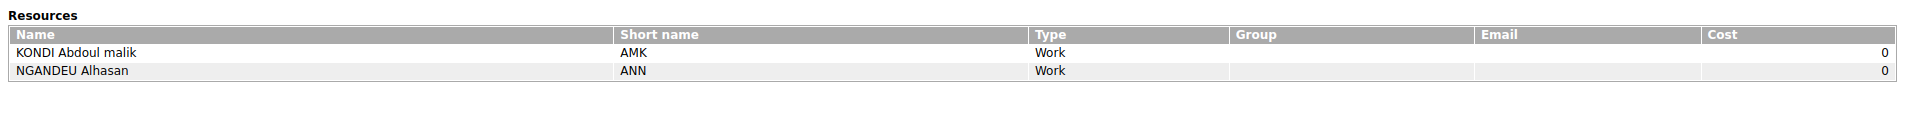
\includegraphics[height=3cm,width=16cm]{images/resources.png}

\section{Résumé des activités}
	Cette semaine pour être franc n'a pas été facile. Les problèmes de santé d'un membre du groupe na pas aidé
	à ce que le travaille soit fait efficacement. néanmoins puisque nous avons un pris de la marge la semaine dernière, 
	on n'a pourra facilement rattraper le coup le semaine prochaine. Ce pendant ce vendredi, nous avons commencer à penser au fonctions que nous allons utilisé et nous avons initialiser un projet \textbf{laravel}. Mais nous avons eu du mal à débuté car nous avions pas trop d'idée de fonctions ou méthodes à part les accesseurs. Voici le diagramme de gant qui montre l'état d'avancement de notre projet.

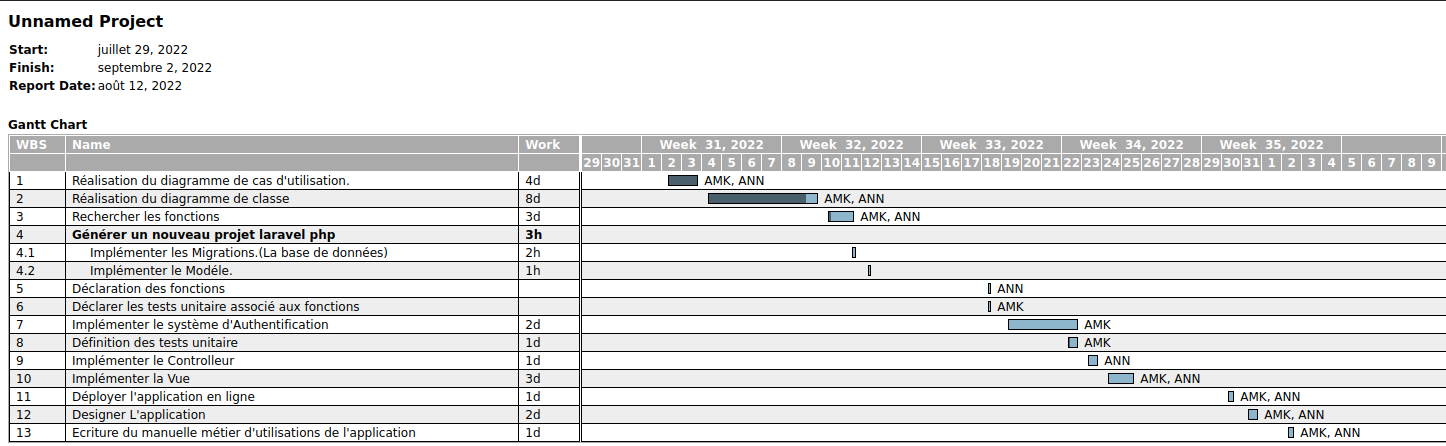
\includegraphics[scale=0.3]{images/jour10.png}

%\section{Détails des événements passé pendant les cinq (5) jour}
%\subsection{Jour 1 : Lundi}

%\newpage
%\subsection{Jour 2 : Mardi}

%\subsection{Jour 3 : Mercredi}

%\subsection{Jour 4 : Jeudi}

%\subsection{Jour 5 : Vendredi}

%\section{Conclusion}
	
\end{document}




